%
%  $Description: Author guidelines and sample document in LaTeX 2.09$
%
%  $Author: ienne $
%  $Date: 1995/09/15 15:20:59 $
%  $Revision: 1.4 $
%
\documentclass[10pt,twocolumn]{article}
\usepackage{latex8}
\usepackage{times}
\usepackage{fancyhdr}
\usepackage{graphicx}
\usepackage{amssymb,amsmath}
\usepackage{listings}
%-------------------------------------------------------------------------
% take the % away on next line to produce the final camera-ready version
\pagestyle{empty}
%-------------------------------------------------------------------------
\begin{document}
\title{Automated Synthesis of Time-Triggered Architecture-based TrueTime Models for Platform Effects Simulation and Analysis}
\author{G. Hemingway, J. Porter, N. Kottenstette, H. Nine, C. vanBuskirk, G. Karsai, J. Sztipanovits\\
Institute for Software Integrated Systems \\ Vanderbilt University\\ 2015 Terrace Place, Nashville, TN 37203 USA\\ graham.hemingway@vanderbilt.edu\\
}
\maketitle
\thispagestyle{fancy}
\renewcommand{\headrulewidth}{0pt}
\lfoot{\footnotesize \parbox{11cm}{978-1-42447074-7/10/\$26.00 �2010 IEEE\\DOI 10.1109/rsp\_2010.43}}
\begin{abstract}
The TrueTime toolbox simulates real-time control systems, including platform-specific details like process scheduling, task execution and network communications.  Analysis using these models provides insight into platform-induced timing effects, such as jitter and delay.  For safety-critical applications, the Time-Triggered Architecture (TTA) has been shown to provide the necessary services to create robust, fault-tolerant control systems.  Communication induced timing effects still need to be simulated and analyzed even for TTA-compliant models.  The process of adapting time-invariant control system models, through the inclusion of platform specifics, into TTA-based TrueTime models requires significant manual effort and detailed knowledge of the desired platform's execution semantics.  In this paper, we present an extension of the Embedded Systems Modeling Language (ESMoL) tool chain that automatically synthesizes TTA-based TrueTime models.  In our tools, time-invariant Simulink models are imported into the ESMoL modeling environment where they are annotated with details of the desired deployment platforms.  A constraint-based offline scheduler then generates the static TTA execution schedules. Finally, we synthesize new TrueTime models that encapsulate all of the TTA execution semantics.  Using this approach it is possible to rapidly prototype, evaluate, and modify controller designs and their hardware platforms to better understand deployment induced performance and timing effects.
\end{abstract}

%-------------------------------------------------------------------------
\Section{Introduction}
Designs for embedded control systems typically start with an ``idealized'', or time-invariant, controller model.  This model usually does not take into account the real-world hardware environment onto which the controller will be deployed.  Deployment of the controller onto actual hardware often introduces temporal effects which may degrade performance or alter the expected behavior of the controller.  Temporal effects can stem from constraints imposed on the controller by the hardware, such as from limited CPU capacity or inadequate communications bandwidth, or from the specific scheduling algorithm used.

Current state-of-the-art model-based controller development environments, such as Simulink/Stateflow \cite{Simulink}, do not directly support the concept of a deployment platform and do not natively simulate the impact of deployment on controller performance.  Third-party extensions to Simulink have been developed that allow these impacts to be simulated and analyzed.  The TrueTime toolbox \cite{ec_99,hca_03} is a suite of Simulink blocks designed expressly for this purpose.  TrueTime supports modeling, simulation, and analysis of distributed real-time control systems including real-time task scheduling and execution, various types of communications networks, and ``analog'' inputs and outputs for interaction with the continuous-time plant model.  While gaining insight into platform effects is crucial, TrueTime imposes an additional burden on systems engineers.  It requires significant effort and a deep understanding of both TrueTime and the desired deployment platform in order to adapt time-invariant models into TrueTime models.

TrueTime's flexibility allows for it to model a wide range of real-time platforms, from simple systems through complex hard real-time architectures.  The Time-Triggered Architecture (TTA) \cite{kopetz_97,kb_02,kg_93} has been shown to provide the necessary services to create robust, fault-tolerant control system communications.  In our interpretation of TTA-based control systems, some of the key architectural requirements are statically scheduled task execution, tight time synchronization between nodes, strongly controlled time-based bus access, and robust support for identifying and handling fault conditions.  TTA provides a fully synchronous distributed environment, at the possible cost of additional time delays between distributed functions. The TrueTime toolbox's primitives have all of the necessary features required to support these concepts, but it does not directly implement a TTA-based platform.

In this paper, we discuss an extension to the Embedded Systems Modeling Language (ESMoL) \cite{pkvnhhts_08, pvknks_09, thibodeaux_08}  tool chain that synthesizes a TTA-based TrueTime model from a system description captured in the ESMoL language.  The ESMoL tool suite is a set of modeling tools for the definition, analysis and synthesis of distributed safety-critical embedded systems.  Its underlying execution semantics closely follow those of TTA platforms.  Designers import software components defined in other tools, such as Simulink or BIP \cite{basu_08, bbs_06}, into an ESMoL model.  Details about the hardware platform are joined with the component definitions into a full description of the embedded system.  From such a system description, the new ESMoL extension can automatically synthesize a TTA-based TrueTime model.

Throughout this paper we use an example to illustrate the steps involved in synthesizing a TrueTime model.  Our example system is an actuator limited quad-integrator model whose corresponding control architecture approximates that of more-advanced architectures used to control quad-rotor aircraft \cite{kp_08} as shown in Fig. \ref{fig:quad_integrator_model}.  
\begin{figure}[ht]
\centering
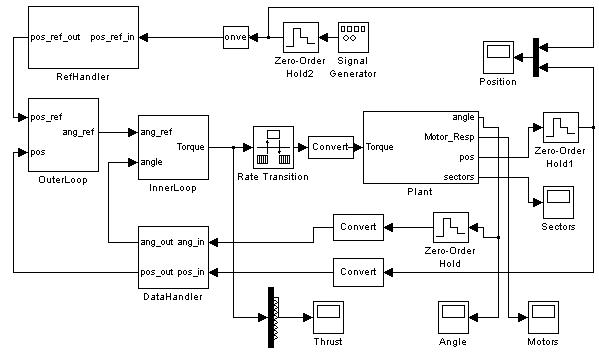
\includegraphics[width=\columnwidth]{figures/quad_integrator.jpg}
    \caption{High-level quad-integrator controller model}
    \label{fig:quad_integrator_model}
\end{figure}

The flight controller is divided into three primary subsystems:
DataHander, InnerLoop and OuterLoop.  The DataHandler block receives
the GPS and IMU sensor data and performs some simple unit conversions.
The InnerLoop controls the first two integrators in the
quad-integrator model which relate a saturated limited control-torque
$|\tau| \leq \tau_{\max}$ to the corresponding 
angular-velocity $\omega(t)=\dot{\theta}(t)$ and angular-position
$\theta$ of a rotational body with inertia $J$ such that
$J\dot{\omega}(t)=\tau(t)$ holds.  In order to control angular-position a
passive discrete-time proportional-derivative controller is
implemented periodically with a zero-order-hold (ZOH) at time $t=kT_s$ 
(in which $T_s$ is the sample-rate and $k$ is an integer) in the 
InnerLoop block such that $\tau(t) = k_p (\theta_d(k) - \theta(k)) - k_d 
\omega(k),\ t\ \in [kT_s,(k+1)T_s)$.  The resulting angular position
is equal to the control force applied to a body with mass $m$ such
that its velocity $v(t)=\dot{x}(t)$ and position $x$ are related such that
$\theta = m \dot{v}$.  Therefore, the OuterLoop control block 
determines the desired angular-position set-point $\theta_d$ to be
sent to the InnerLoop controller using a saturated passive
proportional-derivative controller such that
$\theta_{\mathsf{du}}(k)=k_{\mathsf{po}}(x_d(k)-x(k))
-k_{\mathsf{do}}v(k)$
\begin{equation*}
 \theta_d = \begin{cases}
\theta_{\mathsf{du}},\ \text{ if } |\theta_{\mathsf{du}}| \leq
\theta_{\max}\\
\mathsf{sgn}(\theta_{\mathsf{du}})\theta_{\max},\ \text{otherwise.}
\end{cases}
\end{equation*}
Finally, it is assumed that only $\theta$ and $x$ are periodically
sampled, therefore the respective angular velocity $\omega(k)$ and
velocity $v(k)$ are approximated using the following passive high-pass
filter with roll-off time-constant $\tau_f > 0$:
\begin{equation*}
y(k)-c y(k-1) = \frac{1-c}{T_s}(u(k)-u(k-1)),\ c=\exp(-\frac{T_s}{\tau_f})
\end{equation*}
in which $(u(k),y(k))$ correspond to either $(\theta(k),\omega(k))$ or
$(x(k),v(k))$ respectively.  All three of these subsystems are
incorporated into the final TrueTime model.  The continuous-time plant
and trajectory reference(RefHandler) are also necessary in the
TrueTime model, but reside outside of the  TrueTime blocks.

The remainder of this paper is organized as follows: Section 2 discusses the steps necessary to prepare the model for TrueTime generation.  Section 3 describes the process and results of generating the TrueTime model.  Section 4 covers related work and Section 5 concludes the paper.
\Section{ESMoL Modeling Process}
The ESMoL modeling tools support the entire process of creating embedded systems software, as described in \cite{pvknks_09}.  An understanding of the steps involved in importing and annotating an ESMoL model to prepare it for TrueTime generation is important.  The complete process for modeling and generation includes the following steps: (1) Import controller design from Simulink (2) Define components and message types (3) Generate component functional code (4) Create deployment hardware configuration (5) Deploy components and messages (6) Calculate time-triggered schedule (7) Synthesize the TrueTime model.

The first step for our example is importing the source controller model from Simulink into the ESMoL modeling environment.  The dataflow semantics of the original Simulink model are preserved and are fully represented within the ESMoL model.  Software components in ESMoL are defined by creating references to Simulink subsystem blocks and to input and output message types.  Instances of these software components correspond to individual run-time tasks.  Each task has logical execution time semantics \cite{hhk_01}, which means that all input messages are available before a task consuming them is released, and output messages of the task are sent at precisely defined points in time, after the task has finished.  Message types and their data elements must also be defined.

Once components and message types are defined, a model interpreter synthesizes platform-independent functional code.  The internal dataflow representation of each component is converted into synchronous C-code blocks which will be executed on top of a thin virtual machine that implements the TTA execution semantics. As will be discussed in Section 3, this functional C-code is complied together with a layer of generated ``glue code'', acting as the TTA virtual machine, and together they are directly incorporated into the TrueTime model.

The next step is to define the deployment platform hardware configuration.  In our example the deployment platform consists of a Gumstix Verdex embedded processing module with a Robostix I/O expansion board, as shown in Fig. \ref{fig:platform}.  They are connected via an $I^{2}C$ bus over which time-triggered communications are sent.
\begin{figure}[ht]
\centering
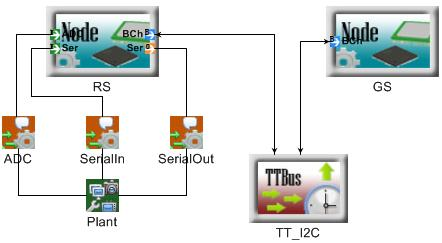
\includegraphics[width=\columnwidth]{figures/platform.jpg}
    \caption{Robostix-Gumstix platform with time-triggered communications bus}
    \label{fig:platform}
\end{figure}

Next, instances of software components are mapped onto the platform.  This step defines the deployment of software onto hardware.  Multiple instances of a particular component may be deployed.  Messages are mapped to I/O ports on the hardware to define channels via which they will be communicated.  The deployment model is used to determine the configuration of TrueTime kernel and network blocks and their relationship and interaction with the plant model.  The deployment of our example quad-rotor components onto our hardware platform is shown in Fig. \ref{fig:deployment}.
\begin{figure}[ht]
\centering
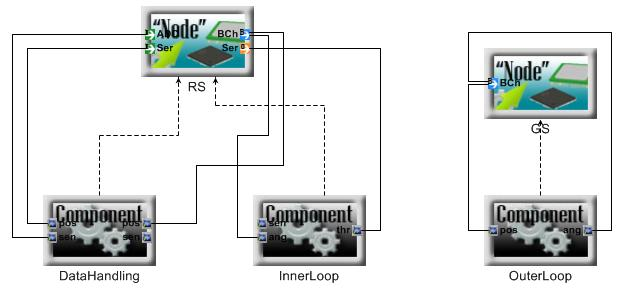
\includegraphics[width=\columnwidth]{figures/deployment.jpg}
    \caption{Deployment of components onto hardware and mapping of ports to communication channels}
    \label{fig:deployment}
\end{figure}

The final step necessary before a TrueTime model can be generated is to execute an off-line schedulability analysis.  Automated schedulability analysis begins with the transformation of the ESMoL model into a scheduler configuration file.  The configuration file contains an abstract version of the design, limited to information about platform connectivity, assignment of tasks to processors, routing of messages through buses, and timing specifications. The ESMoL static scheduler\cite{pks_09} uses this abstract specification to build a finite-domain integer constraint problem, which is solved using the Gecode constraint logic programming library\cite{tools:gecode}.  Details about the scheduler are documented in \cite{pks_09}, though the approach is a refinement of the constraint formulation first described by Schild and W{\"u}rtz\cite{sched:offline}.

The constraint problem models dependencies between tasks and messages, exclusive use of processors and buses, and timing constraints (i.e., maximum acceptable latency between tasks).  If the problem is feasible then a solution will satisfy the specified timing requirements and will contain start times for each of the tasks and messages.  Another automated tool writes the schedule start times to fields in the original model, so that start time information can be used during platform-specific code generation steps.  Infeasible problems are reported as such.

Once a source controller has been imported, components and message types defined, the component functional code generated, a deployment hardware configuration created, components and messages deployed and a time-triggered schedule created, then the ESMoL model is prepared to have the TrueTime model synthesized.
\Section{TrueTime Model Generation, Simulation and Analysis}
There are two primary phases involved in synthesizing a TrueTime model from an ESMoL model.  First, a new Simulink model containing TrueTime network and kernel blocks must be generated.  These kernel blocks only provide a scheduling and execution framework but do not implement task behaviors themselves.  Therefore, code implementing tasks that will execute within kernel blocks must be supplied.  The second phase synthesizes some ``glue code" that, when compiled with the previously generated functional code, see Section 2 step 3, implements the tasks the TrueTime model will execute.

The first phase, creating the new Simulink model, is itself a two step process since, due to available Matlab APIs, it is easier to synthesize an M-file script, which in turn generates a Simulink model, than it is to generate a Simulink model directly.  Once generated, the M-file script is run and a new Simulink model is created with the appropriate configuration of blocks.  A one-to-one correspondence exists between ESMoL nodes and buses and TrueTime kernels and networks respectively.  The original Simulink model's plant and reference signal blocks must also be part of the new model.  Fig. \ref{fig:truetime_model} shows the resulting Simulink model generated from the M-file script.
\begin{figure}[ht]
\centering
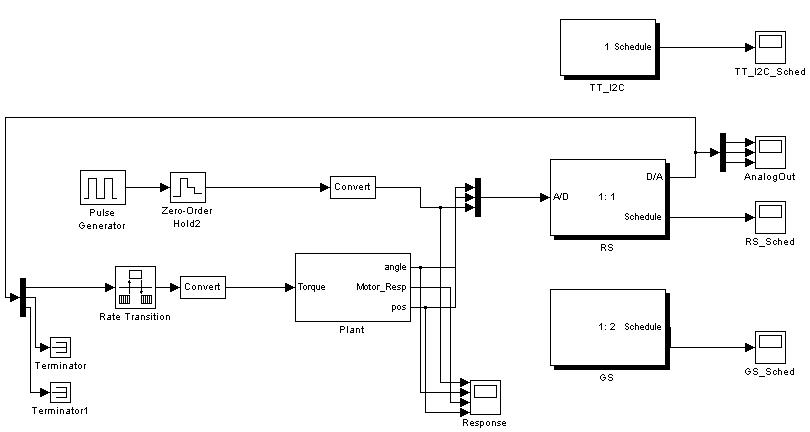
\includegraphics[width=\columnwidth]{figures/truetime.jpg}
    \caption{Synthesized TrueTime model of the quad integrator system}
    \label{fig:truetime_model}
\end{figure}
TrueTime kernels interact with the rest of the Simulink model via ``analog'' inputs and outputs.  Interactions directly between kernels are communicated using the TrueTime network block.  In our example, analog inputs are generated by the ADC and SerialIn blocks and outputs are sent to the SerialOut block, as seen in Fig. \ref{fig:platform}.  The number and ordering of analog signals must be derived from the sensor and actuator messages defined in the ESMoL deployment configuration, as seen in Fig. \ref{fig:deployment}.  Other kernel parameters such as the node number (for network identification) and initial local clock values are similarly derived from the ESMoL model.

The TrueTime network block also must be configured, but does not require any additional code for proper execution.  TrueTime supports a range of networks types: CSMA, Round Robin, FDMA, TDMA, Switched Ethernet, FlexRay, and PROFINET.  Each of these network types must be configured with bus speed, frame size, loss probability, etc.  In our example, a TDMA network block is generated and its properties are configured according to the bus information in the ESMoL model.  A TDMA network was chosen since it implements TTA-like time-based bus access and its timing behavior most resembles that of our $I^{2}C$ bus.

The second phase of creating a TrueTime model is to synthesized the layer of glue code that binds the functional code to the TrueTime run-time.  TrueTime is able to compile and link with either M-file or C/C++ code for task implementations.  In ESMoL both representations of tasks are available, M-file from the original imported controller model, and C-code from the synthesized functional code.  We have chosen to leverage the C functional code since it is identical to the code that will eventually be utilized in a fully deployed control system application.

It is the glue code that implements the semantics of a time-triggered architecture on top of the TrueTime primitives.  TrueTime kernels support both periodic and sporadic execution of tasks.  Neither of these provide the exact timing semantics desired for TTA as they are deadline or period driven and are not guaranteed to begin execution at a specific time.  Given a static TTA execution schedule, tasks should begin execution at their scheduled times.  This requirement necessitates a custom execution scheduler be built on top of the TrueTime scheduler.  This is analogous to implementing a TTA virtual machine on top of a host OS, as discussed in \cite{pvknks_09}.
\begin{figure}[ht]
\centering
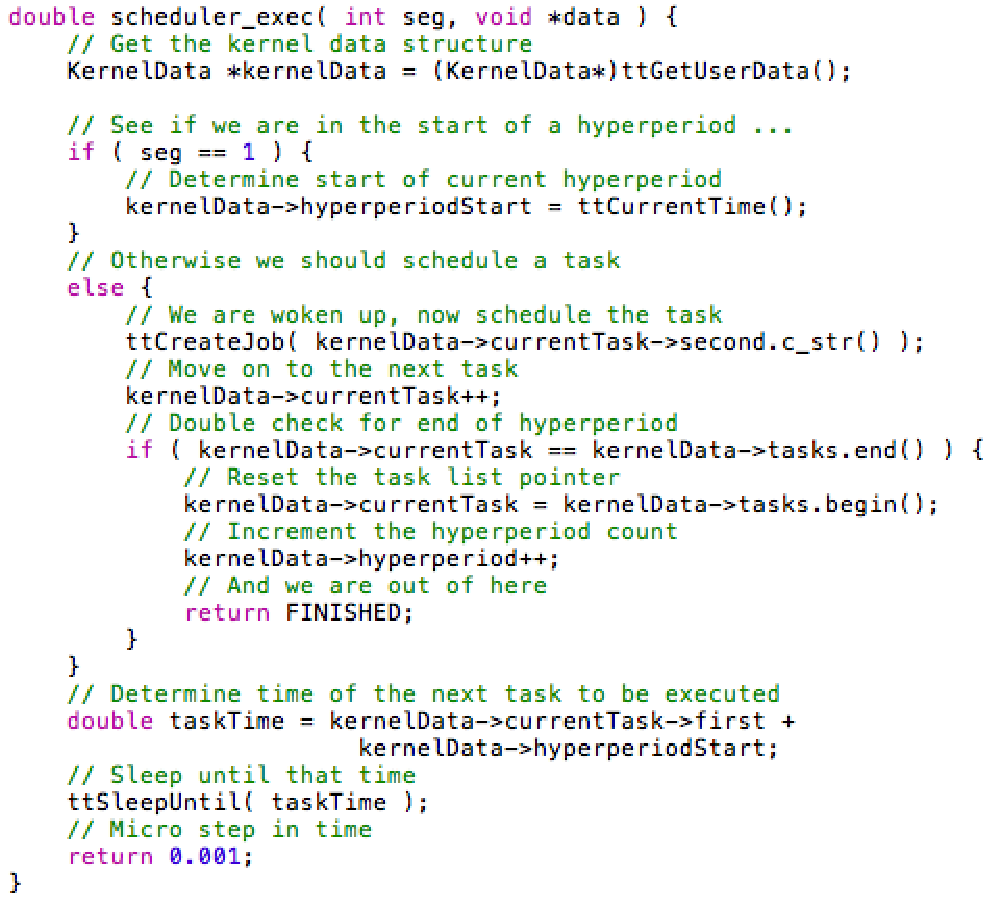
\includegraphics[width=\columnwidth]{figures/scheduler.pdf}
    \caption{Online TTA-based scheduler embedded within each TrueTime kernel}
    \label{fig:scheduler}
\end{figure}
The scheduler used within an ESMoL TTA-based TrueTime model is shown in Fig. \ref{fig:scheduler}.  Our scheduler is implemented as a high-priority periodic task and is scheduled for execution at the beginning of every hyperperiod. TrueTime structures task execution into ``segments''.  A TrueTime task can execute in one or more segments, each of which consumes some finite amount of simulation-clock time.  At the end of each segment the task returns control to the TrueTime scheduler and informs TrueTime of its execution duration via a returned double value.  Any data that must persist between segments or executions must be stored and retrieved in ``UserData'' via TrueTime access functions.

Segment 1 in our scheduler corresponds to the first segment of each execution, and thus the beginning of each hyperperiod.  Our scheduler maintains a sorted map of start times to ESMoL tasks and a pointer that points to the next task to be executed according to this schedule.  During segment 1 the first ESMoL task for the hyperperiod is found and its absolute start time calculated.  The scheduler then sleeps until this time is reached.

When the time has arrived for an ESMoL task to be executed our scheduler should be awoken from sleep by TrueTime.  This corresponds to any segment greater than 1.  ESMoL tasks are implemented as sporadic TrueTime tasks that have a priority lower than our scheduler task.  Our scheduler executes an ESMoL task by scheduling it for execution in TrueTime using the $ttCreateJob()$ function.  Since TrueTime is set to use a priority based scheduling scheme, and no other tasks besides our scheduler are active, as soon as our scheduler ends its segment this new job will execute.  This approach ensures that an ESMoL task starts execution at its statically scheduled time.  ESMoL tasks interact with the TrueTime runtime using segments also.
\begin{figure}[htb]
\centering
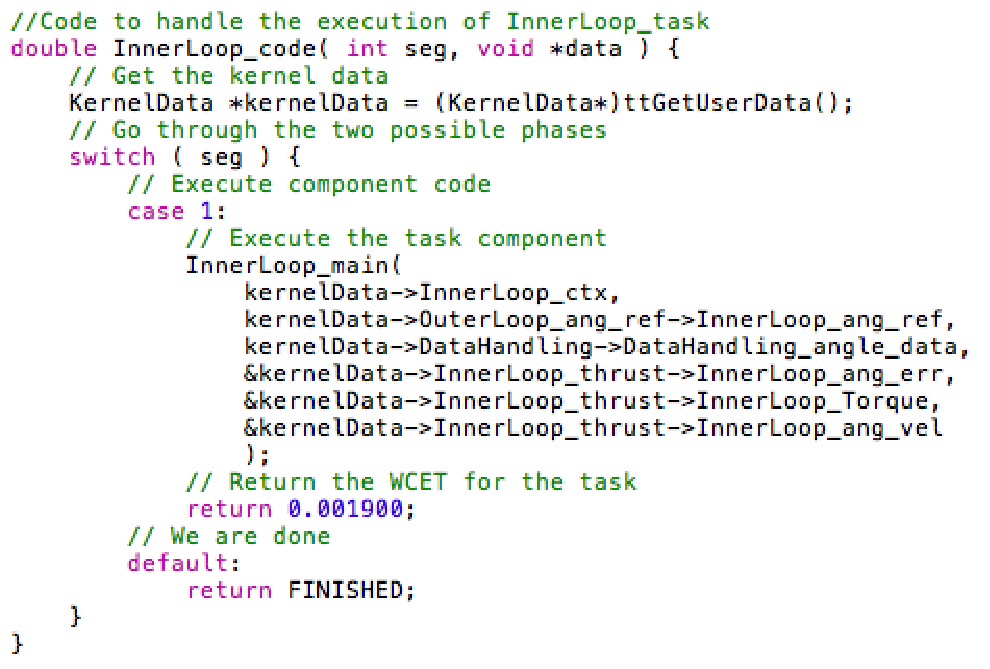
\includegraphics[width=\columnwidth]{figures/task_exec.pdf}
    \caption{InnerLoop component execution code within the TrueTime model}
    \label{fig:task_exec}
\end{figure}
Fig. \ref{fig:task_exec} shows the corresponding code that is invoked when the InnerLoop component is executed.  ESMoL task executions are always contained in a single segment.  All input and output messages are implemented as generated structures contained within the user data context.  The ESMoL task simply calls to the corresponding functional code method that was generated for that task, passing in input data values and pointers to output data locations.  This approach for input and output messages adheres to the logical execution time semantics mentioned in Section 2.  The segment finishes by returning the expected worst-case execution time (WCET) for that task given in the ESMoL model.  TrueTime will always try to let the task execution continue by calling it again with a segment value of 2, but the task will signal it has completed executing by returning the TrueTime defined value FINISHED.

When our scheduler finds no more tasks to execute in a hyperperiod it signals TrueTime that it has completed execution by returning FINISHED.  This cycle is repeated each hyperperiod until the overall simulation is halted.  TrueTime provides output ports on each kernel block that chart the execution states of all tasks.  Fig. \ref{fig:rs_schedule} shows one hyperperiod of execution for the RS node.
\begin{figure}[ht]
\centering
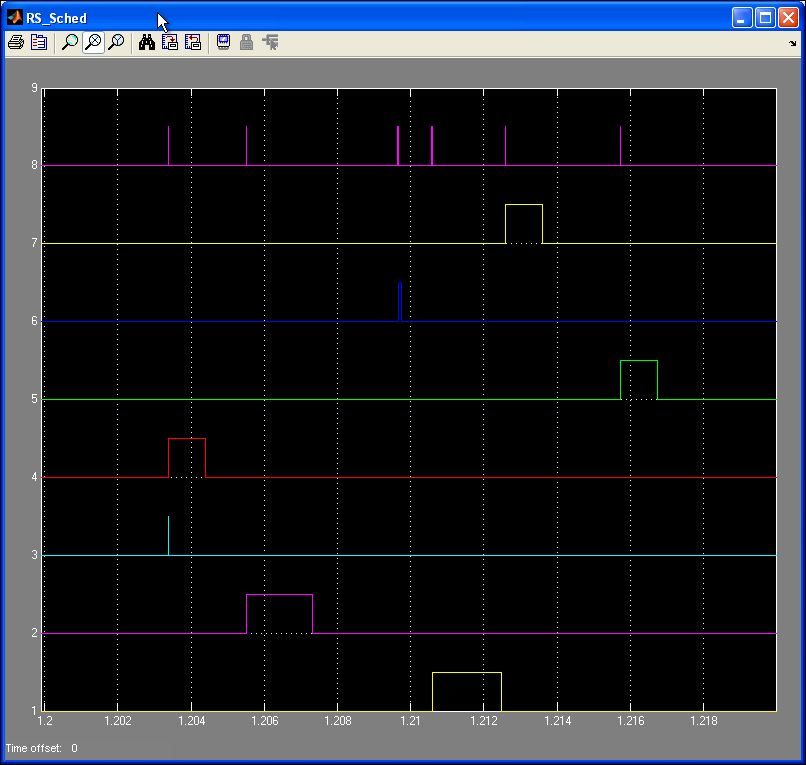
\includegraphics[width=\columnwidth]{figures/rs_schedule.jpg}
    \caption{A single hyperperiod of the task execution schedule for the RS node}
    \label{fig:rs_schedule}
\end{figure}
The top line in the chart is the ESMoL scheduler while all lines below it are individual ESMoL tasks.  For our example there are seven tasks that are executed on the RS node every hyperperiod.  One each for the DataHandler and InnerLoop components.  One for each analog input, ADC and SerialIn, and output, SerialOut.  Finally, there is also a separate task for each message sent or received over the network.  In this case, one message is sent from the RS node to the GS node and one received back.  This ensures that all network communications remain accurate to the TTA semantics.

The purpose of the TrueTime model is to allow designers to simulate and analyze deployment platform induced effects on their controllers.  Fig. \ref{fig:quadintegrator_results}(a) shows the position output of the time-invariant Simulink model compared to the synthesized TrueTime model, and (b) shows the thrust commands (top) and TrueTime model error (bottom).
\begin{figure}[t]
\centering
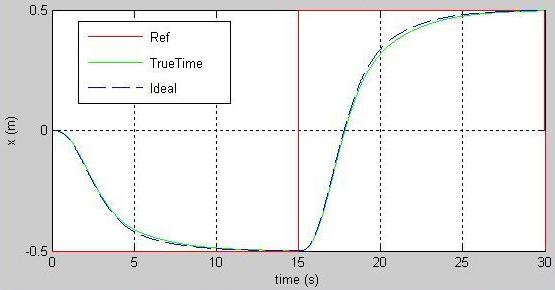
\includegraphics[width=\columnwidth]{figures/results.jpg}
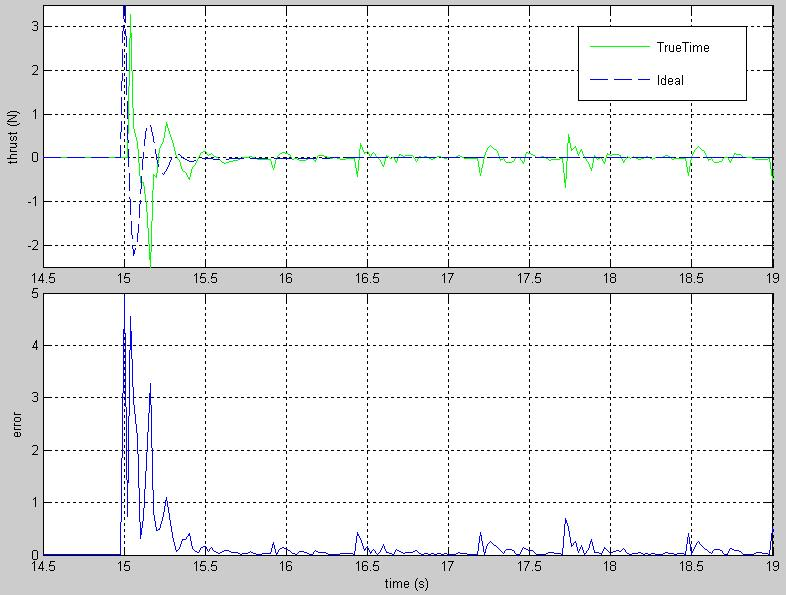
\includegraphics[width=\columnwidth]{figures/results2.jpg}
    \caption{(a) Position tracking (b) Thrust command comparison and (c) TrueTime error}
    \label{fig:quadintegrator_results}
\end{figure}
The time-invariant Simulink model does not contain any delays between the DataHandler, InnerLoop, and OuterLoop subsystems, therefore these blocks calculate output synchronously given input from the Reference signal and the plant blocks.  In contrast, the TrueTime model has propagation delays introduced by the deployment of its components onto hardware and the communications between components.  The schedule causes a total of two hyperperiods to elapse between an input and its associated output response.  The TrueTime model tracks position well, but does introduce nominal variance in the thrust output.  From the tracking we see that this variance does not destabilize the system.

\Section{Related Work}
Several modeling frameworks for real-time embedded systems development include some variant of simulation and analysis of platform effects.  Both SystemC \cite{grotker_02} and AADL \cite{hf_07} are textual languages for defining both software components and their deployment hardware platform.  Similarly, the Metropolis modeling framework \cite{bwhlps_03} aims to give designers tools to create verifiable system models, and has the ability to simulate software components deployed on a defined hardware platform.  None of these modeling frameworks explicitly support the time-triggered architecture.  Additionally, ESMoL differs from AADL, SystemC, and Metropolis in the basic modeling approach\cite{pkvnhhts_08}.  The DECOS project \cite{hsslhbcllss_07} has many similar goals to ESMoL, but the project no longer appears to be active.

Other embedded system modeling frameworks adhere to a time-triggered architecture, such as SCADE\textbackslash Lustre \cite{ccmstn_03}, Giotto \cite{hhk_01} or its successor the Timing Definition Language (TDL) \cite{ffpt_05}, but tend not to include modeling of the deployment hardware platform.  Without native inclusion of both software and hardware components simulation and analysis of platform effects can be difficult or incomplete.

The BIP \cite{basu_08, bbs_06} tool chain supports modeling of heterogenous embedded systems.  The real-time variant of its runtime engine supports timed execution of components, and is able to simulate platform effects as long as a detailed model of the platform is integrated into the overall model.  The BIP language specification \cite{bipUserManual} has not yet been extended to explicitly include concepts for platform definition.

There are numerous examples of TrueTime being used to simulate platform effects \cite{coh_07,vv_05}.  In all of these examples the models are manually created and details of the hardware platforms are translated into TrueTime blocks by hand.  Additionally, no examples were found where time-triggered communication was employed to provide a more robust distributed control system architecture.
\Section{Future Work and Conclusion}
Some aspects of TTA are not yet fully represented in the synthesized TrueTime models.  Redundant communication networks, membership services and time synchronization are important services required for robust execution and fault-tolerance.  Future work will expand the current focus of TrueTime models to include better modeling of fault conditions and the impact faults may have on controller performance.  Time synchronization between nodes is an important aspect of TTA, but is somewhat moot in Simulink/TrueTime since all nodes can rely upon the global simulation clock.  We plan on enhancing our TrueTime models to incorporate a time synchronization protocol and to allow local clocks on nodes to have some drift and error from the global simulation clock.  Together, these enhancements should allow our TrueTime models to more accurately reflect TTA behavior.

Inclusion of sporadically executed tasks into the static schedule is also an interesting research direction.  Some existing TTA-based approaches allow limited execution of tasks outside of the static task schedule.  Support for sporadic execution will require extending both our online scheduler and our communications network interfaces.

In this paper we presented an extension to the ESMoL tool chain for synthesizing TTA-based TrueTime models.  Automatic synthesis via the tool chain greatly reduces the level of effort needed to create TrueTime models.  Leveraging TrueTime for system prototyping is useful compared to generating code directly for the embedded platform because it is far easier to explore and debug execution behavior, alter model design, or tap data streams in TrueTime/Simulink than it is with C-code loaded onto an actual embedded system.  Once system behavior has been analyzed and design criteria have been met in TrueTime the final transition to deploying onto an embedded platform is eased.
\Section{Acknowledgements}
This work was sponsored (in part) by the Air Force Office of Scientific Research, USAF, under grant/contract number FA9550-06-0312.  The views and conclusions contained herein are those of the authors and should not be interpreted as necessarily representing the official policies or endorsements, either expressed or implied, of the Air Force Office of Scientific Research or the U.S. Government.

\bibliographystyle{latex8}
\bibliography{RSP10}
\end{document}

